\documentclass[conference]{IEEEtran}
\IEEEoverridecommandlockouts
\usepackage{cite}
\usepackage{amsmath,amssymb,amsfonts}
\usepackage{algorithmic}
\usepackage{graphicx}
\usepackage{textcomp}
\usepackage{xcolor}
\usepackage{booktabs}
\usepackage{multirow}
\usepackage{url}

\begin{document}

\title{Federated Reinforcement Learning for Smart Multi-Intersection Traffic Signal Control: A Standardized Benchmarking Framework}

\author{\IEEEauthorblockN{Majid Ibrahim}
\IEEEauthorblockA{\textit{College of Information Technology} \\
\textit{United Arab Emirates University}\\
Al Ain, UAE}
\and
\IEEEauthorblockN{Hamdan Al Mehairbi}
\IEEEauthorblockA{\textit{College of Information Technology} \\
\textit{United Arab Emirates University}\\
Al Ain, UAE}
\and
\IEEEauthorblockN{Abdallah Al Falasi}
\IEEEauthorblockA{\textit{College of Information Technology} \\
\textit{United Arab Emirates University}\\
Al Ain, UAE}
\and
\IEEEauthorblockN{Mohammad Al Blooshi}
\IEEEauthorblockA{\textit{College of Information Technology} \\
\textit{United Arab Emirates University}\\
Al Ain, UAE}
\and
\IEEEauthorblockN{Mohamed Al Rayassi}
\IEEEauthorblockA{\textit{College of Information Technology} \\
\textit{United Arab Emirates University}\\
Al Ain, UAE}
}

\maketitle

\begin{abstract}
Reinforcement learning (RL) has shown strong potential for adaptive traffic signal control, yet existing studies compare training strategies under inconsistent experimental setups, making it impossible to attribute performance differences to the strategy itself. This paper presents a standardized benchmarking framework that evaluates three RL training strategies---single-agent RL (SARL), multi-agent RL (MARL), and federated RL (FedRL)---for multi-intersection traffic signal control under identical controlled conditions. The framework holds eight experimental layers constant (simulator, network topology, traffic demand, observations, reward, algorithm, training budget, and evaluation protocol), isolating the training strategy as the sole independent variable. We introduce a 14-feature intersection-agnostic observation space that enables federated weight sharing across heterogeneous intersection types, and a reward-weighted aggregation scheme that prioritizes high-performing intersections during model averaging. Preliminary results on two synthetic SUMO grid topologies (3$\times$3 and 5$\times$5) show that all RL strategies reduce average waiting time by 73--82\% compared to fixed-time control, while FedRL achieves comparable performance to centralized approaches with 39\% less communication cost. Notably, FedRL's advantage over SARL increases with network size, suggesting that federation becomes more valuable as the number of intersections grows.
\end{abstract}

\begin{IEEEkeywords}
federated learning, reinforcement learning, traffic signal control, multi-agent systems, benchmarking, PPO, SUMO
\end{IEEEkeywords}

\section{Introduction}

Traffic congestion cost the United States approximately \$87 billion in 2019 alone in lost productivity and fuel waste \cite{b_inrix}. Most urban traffic signals still operate on fixed-time schedules with no awareness of real-time conditions. Reinforcement learning (RL) offers a promising alternative by training signal controllers to adapt their timing based on observed traffic states \cite{b_wei_survey}.

Three distinct approaches have emerged for organizing RL-based traffic control across multiple intersections. Single-agent RL (SARL) trains one shared policy that receives observations from all intersections. Multi-agent RL (MARL) assigns independent policies to each intersection with centralized coordination. Federated RL (FedRL) trains local policies independently and periodically aggregates model weights through a central server, reducing communication overhead while enabling knowledge sharing \cite{b_fedlight, b_seal}.

Despite growing interest, the literature lacks a fair comparison of these strategies. Each study uses different simulators, observation representations, reward functions, and evaluation protocols. When two papers report different results, it is unclear whether the difference stems from the training strategy or the experimental setup. Existing benchmarks such as RESCO \cite{b_resco} compare RL algorithms but do not evaluate federated training strategies. LibSignal \cite{b_libsignal} compares simulators but not training strategies. No standardized framework exists for comparing how policies are organized across intersections.

This paper makes the following contributions:
\begin{itemize}
    \item A benchmarking framework that controls eight experimental layers, isolating training strategy as the sole independent variable.
    \item A 14-feature intersection-agnostic observation space that enables federated weight sharing across heterogeneous intersection types.
    \item A reward-weighted federated aggregation scheme where better-performing intersections contribute proportionally more to the global model.
    \item Empirical evidence that the optimal training strategy depends on network size, with FedRL's advantage increasing as the number of intersections grows.
\end{itemize}

\section{Related Work}

\subsection{RL for Traffic Signal Control}

Wei et al.\ \cite{b_wei_survey} survey RL-based traffic signal control methods, identifying inconsistencies in experimental setups across studies. Ault and Sharon \cite{b_resco} introduced RESCO, a benchmark comparing IDQN, IPPO, MPLight, and FMA2C on real-world SUMO networks from Cologne and Ingolstadt. However, RESCO evaluates different RL algorithms rather than different training strategies, and does not include any federated approaches. LibSignal \cite{b_libsignal} standardizes evaluation across simulators (SUMO and CityFlow) but similarly omits federated strategies and communication cost analysis.

\subsection{Federated RL for Traffic}

Ye et al.\ \cite{b_fedlight} proposed FedLight, the first application of federated learning to traffic signal control, using A2C on a single grid topology. However, FedLight was not compared against non-federated baselines under identical conditions, making it difficult to assess the value added by federation. Hudson et al.\ \cite{b_seal} introduced the SEAL framework with intersection-agnostic observations and communication cost analysis, but evaluated only pre-trained weights without training from scratch and compared only against fixed-time control. Bao et al.\ \cite{b_bao} explored partial model aggregation with DQN, but used different reward functions and observation representations, making results incomparable to other studies. Fu et al.\ \cite{b_hfrl} proposed hierarchical federated RL with clustering, using real-world NYC data, but focused on a single aggregation variant.

Our aggregation mechanism builds on FedAvg \cite{b_fedavg} with reward-weighted modifications, and we evaluate FedProx \cite{b_fedprox} as an aggregation variant for handling heterogeneous intersection data distributions.

These works each contribute valuable insights. However, because they evaluate under different conditions---different algorithms, different observations, different rewards---no direct comparison between SARL, MARL, and FedRL has been possible. Our framework addresses this gap.

\section{Methodology}

\subsection{System Architecture}

Fig.~\ref{fig:architecture} illustrates the overall system architecture. SUMO communicates with the environment layer through TraCI, which computes the 14-feature observation vector and reward signal. The PPO agent receives observations and produces actions. The training strategy layer determines how policies are organized---this is the only component that differs between SARL, MARL, and FedRL.

\begin{figure*}[htbp]
\centerline{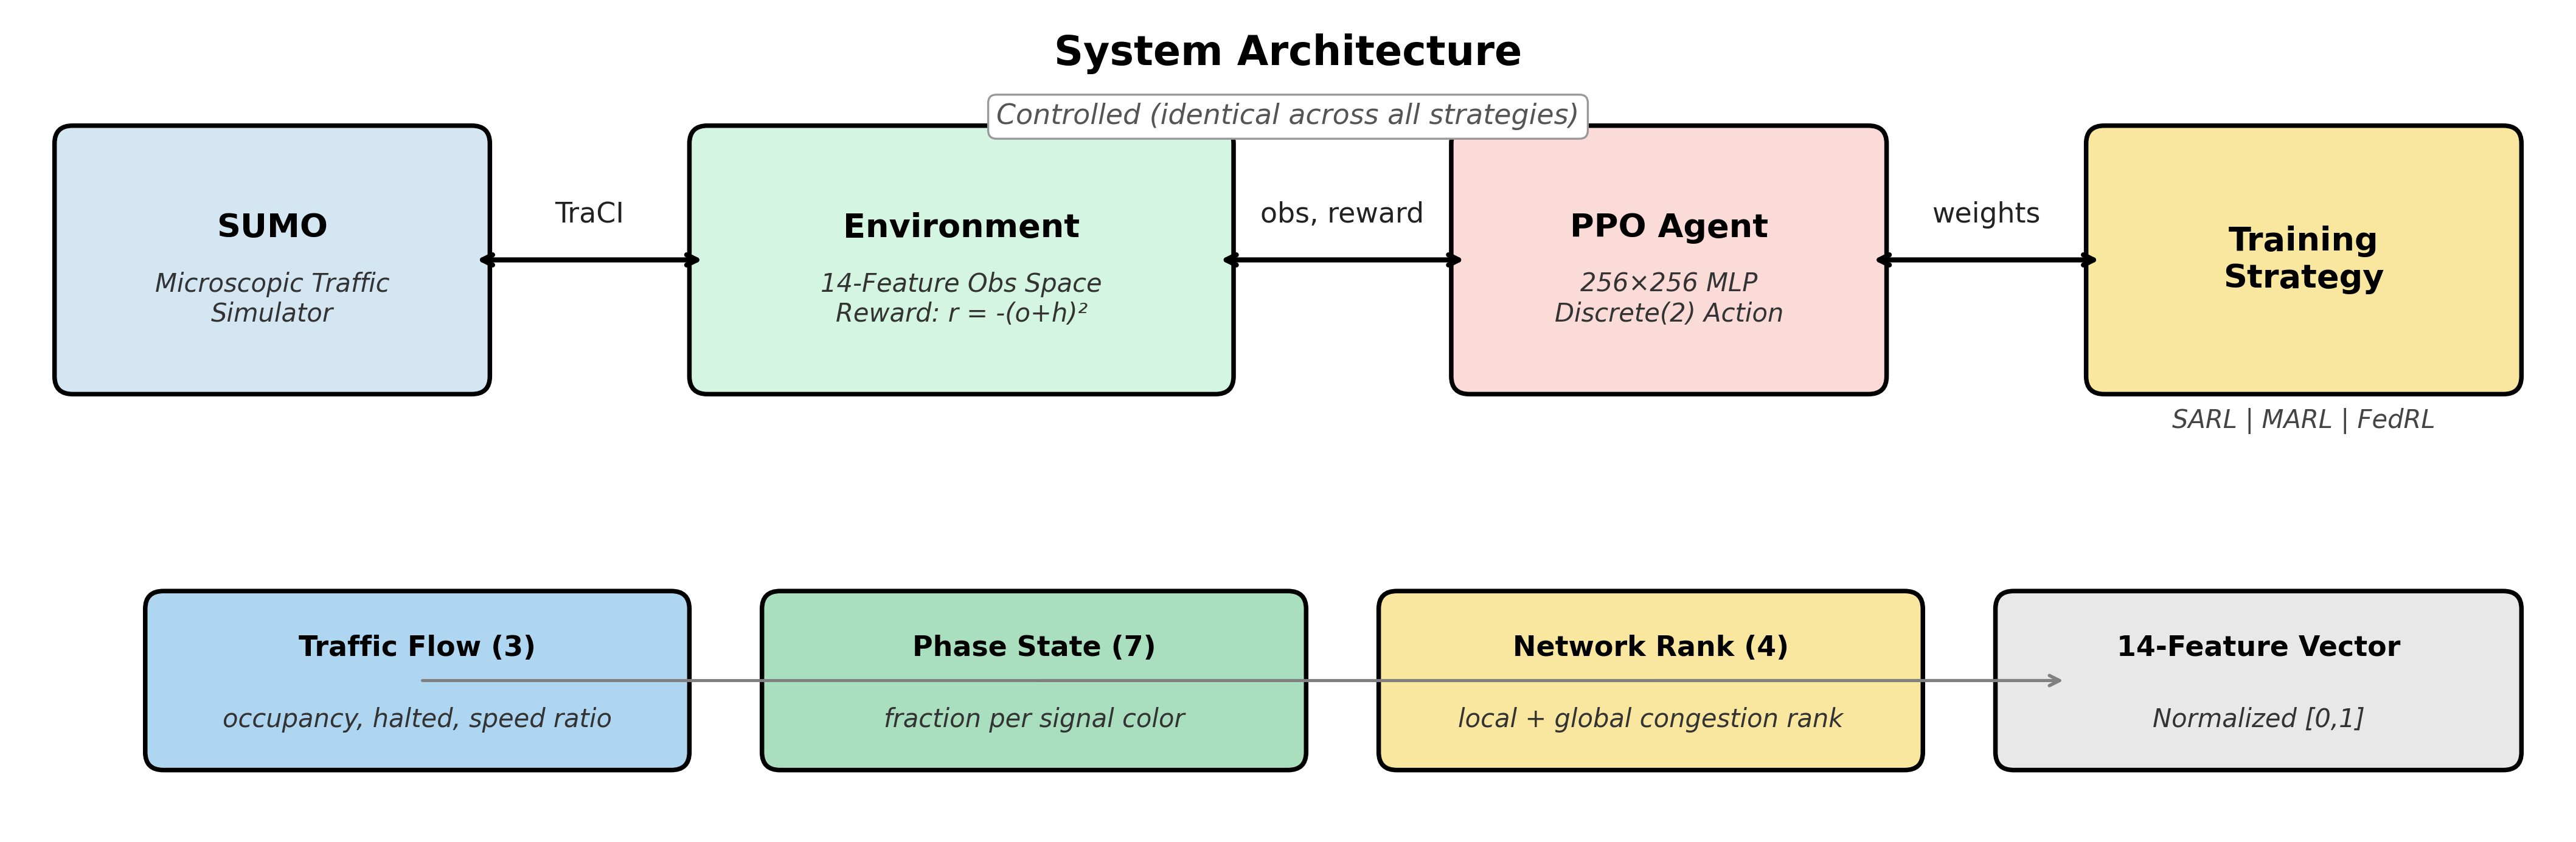
\includegraphics[width=0.85\textwidth]{figures/fig_architecture.png}}
\caption{System architecture. The environment, observation pipeline, and PPO agent are identical across all strategies (controlled variables). Only the training strategy layer varies (independent variable). The observation pipeline converts raw TraCI data into a 14-feature normalized vector through three feature groups: traffic flow (3), phase state (7), and network rank (4).}
\label{fig:architecture}
\end{figure*}

\subsection{Benchmarking Framework}

The core principle of our framework is that a fair comparison requires controlling all variables except the one under test. We organize our experimental design into three categories:

\textbf{Controlled variables (held constant):} road network topology (.net.xml), traffic demand (360 VPLPH, same random seeds), observation function (14-feature intersection-agnostic vector), action space (Discrete(2)), reward function ($r = -(o + h)^2$), RL algorithm (PPO with identical hyperparameters), training budget (25 episodes), and evaluation protocol (5 Monte Carlo runs, seeds 42--46).

\textbf{Independent variable:} how policies are organized across intersections---one shared (SARL), independent per-intersection (MARL), or per-intersection with periodic federated aggregation (FedRL).

\textbf{Dependent variables:} average waiting time (s), average travel time (s), and communication cost (MB).

All three strategies share the same codebase. SARL, MARL, and FedRL trainers inherit from a common base class, use the same environment wrapper, and call the same observation and reward computation functions. The divergence is limited to the policy mapping function and the optional aggregation step in FedRL.

\subsection{Simulation Environment}

We use SUMO (Simulation of Urban Mobility) version 1.26.0 \cite{b_sumo}, a microscopic traffic simulator that models individual vehicles with realistic car-following physics (Krauss model). Agent-environment interaction occurs through TraCI (Traffic Control Interface), SUMO's Python API for querying lane occupancy, vehicle speeds, and traffic light states, and for setting traffic light phases at each timestep.

Traffic is generated using SUMO's \texttt{randomTrips.py} with \texttt{--fringe-factor 100} to bias origins and destinations toward network edges, and deterministic seeds for reproducibility. A demand of 360 vehicles per lane per hour (VPLPH) is the standard setting in the SEAL literature \cite{b_seal}, producing moderate congestion without gridlock. On a Grid 3$\times$3 network with 24 lanes, this generates approximately 8,640 vehicles per hour.

\subsection{Observation Space}

A key design requirement for federated aggregation is that all intersection policies must share identical input and output dimensions, regardless of the physical layout of each intersection. We achieve this through a 14-feature intersection-agnostic observation vector, organized into three groups:

\textbf{Traffic Flow (3 features):}
\begin{itemize}
    \item \textit{Lane occupancy} ($o$): sum of vehicle lengths on controlled lanes divided by sum of lane lengths. We use physical vehicle length rather than count because vehicles of different sizes occupy different amounts of road space.
    \item \textit{Halted lane occupancy} ($h$): same computation but only for vehicles with speed below 0.1~m/s. Tracked separately because stopped vehicles cause cascading upstream delays that moving vehicles at the same density do not.
    \item \textit{Speed ratio}: average vehicle speed divided by lane speed limit. Returns 1.0 when no vehicles are present (free flow).
\end{itemize}

\textbf{Phase State (7 features):} The fraction of controlled links showing each SUMO signal state (red, yellow, minor green, priority green, u-turn, off-blinking, off). Encoding as fractions rather than raw phase strings (e.g., ``GGrr'') makes the representation independent of intersection geometry---a 4-lane intersection with ``GGrr'' and a 6-lane intersection with ``GGGrrr'' both produce ``50\% green, 50\% red.''

\textbf{Network Rank (4 features):} Local and global rankings for both total congestion and halted vehicles. Local rank indicates how congested an intersection is relative to its immediate neighbors; global rank indicates its position across the entire network. An absolute occupancy value of 0.8 carries different implications depending on whether the intersection is the most or least congested in the network; ranking features capture this context.

All 14 features are normalized to $[0, 1]$, computed by the same shared code for every strategy.

\subsection{Action Space and Reward Function}

Each agent selects from two actions: keep the current traffic light phase (0) or advance to the next phase in the predefined cycle (1). A binary action space is a necessary condition for federated aggregation across heterogeneous intersections: phase-selection actions (Discrete($N$) where $N$ varies by intersection type) would require different output layer dimensions across intersection types, making it impossible to average model weights. The binary formulation ensures all policies share identical input and output dimensions regardless of the physical intersection layout.

Timing constraints enforce a minimum of 4~seconds between phase changes and a maximum of 120~seconds before a forced change, consistent with FHWA signal timing guidelines.

The reward at intersection $k$ is:
\begin{equation}
    r_k = -(o_k + h_k)^2
    \label{eq:reward}
\end{equation}
where $o_k$ is lane occupancy and $h_k$ is halted lane occupancy. The quadratic form penalizes high congestion disproportionately---going from 20\% to 40\% occupancy costs far less than going from 60\% to 80\%. Halted vehicles appear in both terms intentionally: a stopped vehicle contributes to both $o_k$ (it occupies lane space) and $h_k$ (it is stopped), receiving a larger penalty because it causes more disruption than a moving vehicle at the same density.

\subsection{RL Algorithm}

All strategies use Proximal Policy Optimization (PPO) \cite{b_ppo} with identical hyperparameters: learning rate $5 \times 10^{-5}$, clip parameter 0.3, KL target 0.3, train batch size 4000, SGD minibatch size 128, GAE $\lambda = 1.0$, and VF clip 10. These values are drawn from the SEAL framework \cite{b_seal} and are standard in the traffic RL literature. The policy network is a fully connected MLP with two hidden layers of 256 neurons each and ReLU activation (approximately 70,000 parameters). Training is implemented in Ray RLlib \cite{b_rllib} with \texttt{num\_workers=0} for deterministic single-threaded execution.

Hyperparameters are deliberately not tuned per-strategy. If FedRL received different hyperparameters than MARL, performance differences could not be attributed to the training strategy alone.

\subsection{Training Strategies}

\textbf{SARL (Single-Agent RL):} One shared policy serves all intersections. The policy mapping function maps every agent ID to the same policy: \texttt{lambda \_\,:\,"sarl{-}policy"}. All observations flow to one central model every timestep.

\textbf{MARL (Multi-Agent RL):} Each intersection has its own policy with independent weights. The policy mapping function maps each agent ID to its own policy. A central trainer coordinates gradient updates, requiring continuous communication.

\textbf{FedRL (Federated RL):} Each intersection has its own policy and trains locally. After each episode (every 4000 timesteps), all intersection policies send their weights to a central server. The server computes a reward-weighted average:
\begin{equation}
    w_{\text{global}} = \sum_{k=1}^{N} \alpha_k \cdot w_k
    \label{eq:fedavg}
\end{equation}
where $\alpha_k$ is the normalized contribution coefficient for intersection $k$. Since rewards are negative (more negative = worse), we first shift all rewards to be non-negative by subtracting the minimum reward across intersections, then normalize so that $\sum \alpha_k = 1$. Formally, let $R_k = \sum_t r_k^{(t)}$ denote the accumulated reward for intersection $k$ over the episode. The contribution coefficient is:
\begin{equation}
    \alpha_k = \frac{R_k - R_{\min}}{\sum_{j=1}^{N}(R_j - R_{\min})}
    \label{eq:alpha}
\end{equation}
This ensures intersections with higher (less negative) rewards---i.e., better-performing intersections---contribute proportionally more to the global model. The averaged weights are distributed back to all intersections. Between aggregation rounds, there is no server communication.

We use reward-weighted rather than equal-weight averaging because intersections experience different traffic volumes. A center intersection processing heavy traffic generates a richer training signal than a quiet corner; weighting by reward ensures the most useful knowledge drives the consensus.

\subsection{Evaluation Protocol}

Each trained policy is evaluated using Monte Carlo evaluation: the trained model runs inference (no learning, no exploration) on 5 traffic scenarios generated with seeds 42--46. Each seed generates different vehicle routes and departure times, producing traffic scenarios not seen during training. Metrics are extracted from SUMO's \texttt{tripinfo} XML output, which records actual vehicle waiting time and travel time based on simulation physics. This ensures metrics are simulator-verified rather than computed by our code.

\section{Experimental Setup}

\subsection{Network Topologies}

We evaluate on two synthetic SUMO grid networks:
\begin{itemize}
    \item \textbf{Grid 3$\times$3:} 9 intersections, 24 controlled lanes. Center intersections have more lanes than edge intersections, creating controlled heterogeneity.
    \item \textbf{Grid 5$\times$5:} 25 intersections, 80 controlled lanes. Same heterogeneity pattern at larger scale.
\end{itemize}

Two topologies provide a minimal scalability test. A single topology cannot reveal scaling behavior; two show whether trends hold as the network grows.

\subsection{Training Configuration}

Each configuration trains for 25 episodes, where one episode consists of 450 simulation timesteps (7.5 minutes of simulated traffic). A Grid 3$\times$3 configuration completes in approximately 30 minutes of wall-clock time; Grid 5$\times$5 takes approximately 90 minutes. Convergence was verified by running a separate 50-episode experiment on Grid 5$\times$5, confirming that reward plateaus by episode 20 with no meaningful improvement thereafter. Traffic demand is set at 360 VPLPH across all configurations.

\subsection{Communication Cost Model}

Communication cost is computed theoretically from actual data structure sizes rather than measured on a physical network. The relative ratios between strategies are robust because protocol overhead (TCP/IP headers, encryption) affects all strategies equally. Per-timestep data includes observations (14 floats $\times$ 4 bytes = 64 bytes per intersection), actions (1 byte), and V2I messages (32 bytes). FedRL additionally exchanges model weights ($\approx$50~KB per intersection) once per aggregation round. Detailed calculations are presented in Section~V-E.

\section{Results}

\subsection{Training Convergence}

Fig.~\ref{fig:learning_curves} shows the mean episode reward over 25 training episodes. All three strategies converge successfully on both topologies. FedRL achieves the highest final reward on both grids. On Grid 3$\times$3, SARL converges faster initially because one shared policy receives data from all 9 intersections from the start. However, FedRL overtakes SARL around episode 15 as the aggregation mechanism enables agents to benefit from each other's experience. On Grid 5$\times$5, the gap between FedRL and the other strategies is larger, because each agent individually observes a smaller portion of the overall network dynamics, making shared knowledge through periodic aggregation more valuable.

\begin{figure}[htbp]
\centerline{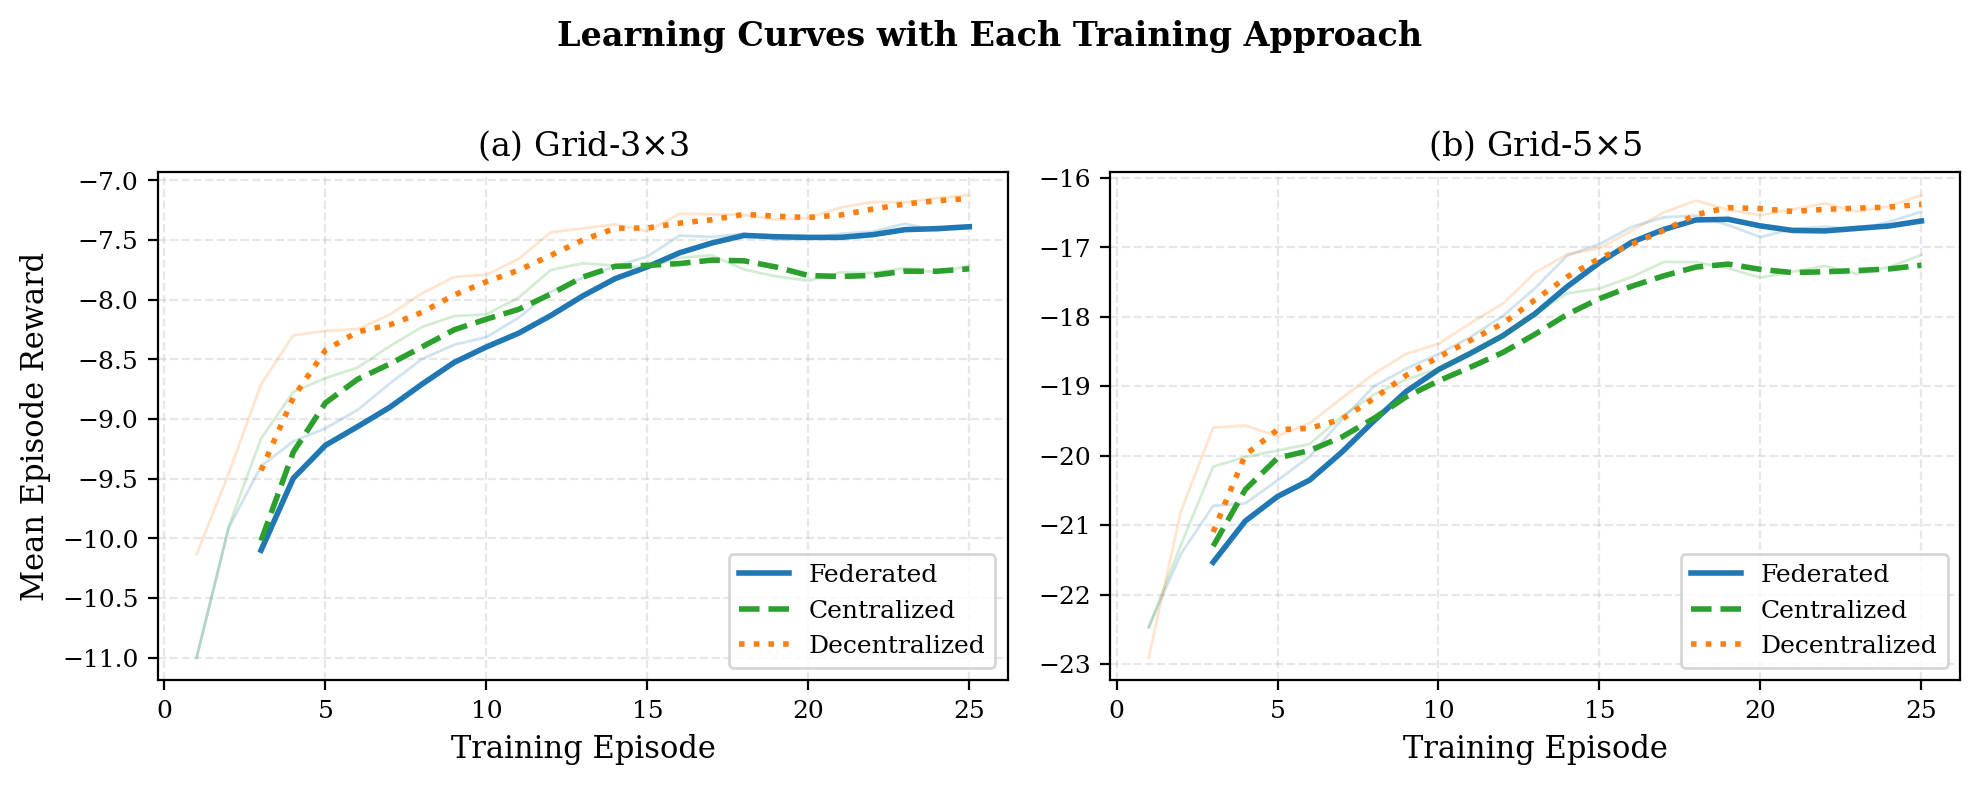
\includegraphics[width=\columnwidth]{figures/fig_learning_curves.png}}
\caption{Learning curves for SARL, MARL, and FedRL on Grid 3$\times$3 (left) and Grid 5$\times$5 (right). FedRL achieves highest reward on both topologies. Faded lines show raw per-episode rewards; solid lines show moving average (window=3).}
\label{fig:learning_curves}
\end{figure}

\subsection{Waiting Time}

Table~\ref{tab:waiting_time} presents average waiting time results from Monte Carlo evaluation. All RL strategies reduce waiting time by 73--82\% compared to fixed-time control, confirming that adaptive signal timing provides substantial improvement over static schedules.

Among the RL strategies, SARL achieves the lowest waiting time on Grid 3$\times$3 (14.2~s vs.\ FedRL's 15.4~s), because one shared policy can efficiently capture the dynamics of a 9-intersection network. On Grid 5$\times$5, FedRL achieves 19.2~s compared to MARL's 24.7~s and SARL's 19.8~s. This reversal demonstrates that the optimal strategy depends on network size---a finding that would be invisible without testing on multiple topologies.

We note that on Grid 3$\times$3, the differences between RL strategies are within one standard deviation (FedRL: 15.4 $\pm$ 1.3, SARL: 14.2 $\pm$ 0.8), suggesting they may not be statistically significant at this sample size. Formal significance testing with Wilcoxon signed-rank tests is planned for the final evaluation with increased Monte Carlo runs.

MARL performs worst among RL strategies on Grid 5$\times$5 because each agent optimizes only for its own intersection with no awareness of neighbors. An agent may clear its own queue by pushing congestion downstream.

\begin{table}[htbp]
\caption{Average Waiting Time (seconds, mean $\pm$ std over 5 MC runs)}
\begin{center}
\begin{tabular}{lcc}
\toprule
\textbf{Strategy} & \textbf{Grid 3$\times$3} & \textbf{Grid 5$\times$5} \\
\midrule
FedRL & 15.4 $\pm$ 1.3 & 19.2 $\pm$ 0.8 \\
MARL & 14.8 $\pm$ 1.5 & 24.7 $\pm$ 1.3 \\
SARL & 14.2 $\pm$ 0.8 & 19.8 $\pm$ 1.1 \\
Fixed-Time & 76.9 $\pm$ 25.7 & 70.6 $\pm$ 22.7 \\
\bottomrule
\end{tabular}
\label{tab:waiting_time}
\end{center}
\end{table}

\subsection{Travel Time}

Table~\ref{tab:travel_time} shows average travel time results, which follow a similar pattern. All RL strategies significantly outperform fixed-time control. FedRL and SARL achieve comparable travel times on Grid 5$\times$5 (84.8~s vs.\ 84.5~s), while MARL lags at 92.1~s.

\begin{table}[htbp]
\caption{Average Travel Time (seconds, mean $\pm$ std over 5 MC runs)}
\begin{center}
\begin{tabular}{lcc}
\toprule
\textbf{Strategy} & \textbf{Grid 3$\times$3} & \textbf{Grid 5$\times$5} \\
\midrule
FedRL & 61.3 $\pm$ 1.6 & 84.8 $\pm$ 1.5 \\
MARL & 60.6 $\pm$ 1.9 & 92.1 $\pm$ 2.4 \\
SARL & 58.8 $\pm$ 0.9 & 84.5 $\pm$ 1.9 \\
Fixed-Time & 117.3 $\pm$ 27.1 & 124.6 $\pm$ 24.0 \\
\bottomrule
\end{tabular}
\label{tab:travel_time}
\end{center}
\end{table}

\subsection{Communication Cost}

Fig.~\ref{fig:comm_cost} presents the communication cost comparison. SARL and MARL transmit 162--485~MB during training due to continuous per-timestep data streaming. FedRL achieves a 39\% reduction (102.6~MB on Grid 3$\times$3, 285.0~MB on Grid 5$\times$5) by replacing continuous observation streaming with periodic model weight exchanges of approximately 50~KB per intersection per episode.

To illustrate the calculation on Grid 3$\times$3: SARL streams 97 bytes (64 observation + 1 action + 32 V2I) per intersection per timestep across 9 intersections and 200,000 timesteps, yielding 174.6~MB. FedRL transmits only V2I messages (32 bytes) per timestep (57.6~MB) plus model weight exchanges of 50~KB $\times$ 9 intersections $\times$ 2 directions $\times$ 50 rounds (45.0~MB), totaling 102.6~MB.

This reduction becomes more significant in deployment scenarios where traffic signal controllers are edge devices communicating over wireless networks with limited bandwidth.

\begin{figure*}[htbp]
\centerline{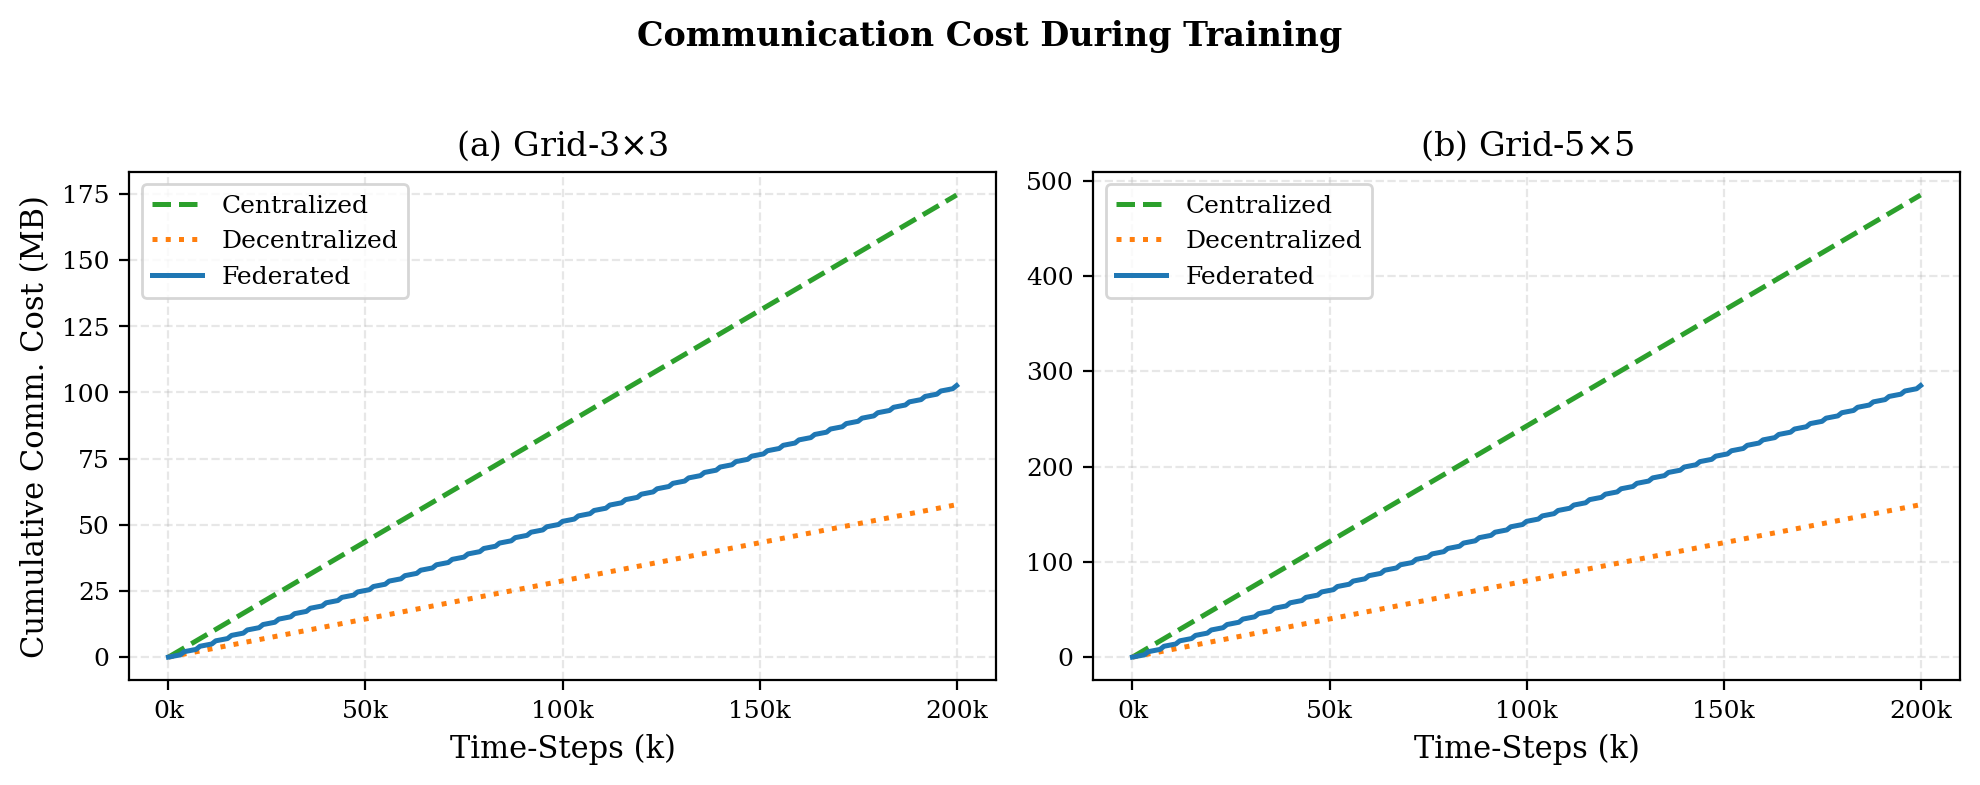
\includegraphics[width=0.7\textwidth]{figures/fig_communication_cost.png}}
\caption{Communication cost during training. FedRL reduces communication by 39\% compared to SARL and MARL by exchanging model weights once per episode instead of streaming data every timestep. Values computed from data structure sizes (64 bytes per observation, 50~KB per model weight exchange).}
\label{fig:comm_cost}
\end{figure*}

\subsection{Trade-off Summary}

Table~\ref{tab:tradeoff} summarizes the trade-offs between strategies based on midterm results. The communication cost and scalability columns are supported by experimental evidence. The ``Best When'' characterizations for SARL and FedRL are supported by the observed reversal between Grid 3$\times$3 and Grid 5$\times$5. MARL's characterization remains tentative pending multi-demand evaluation, as it underperformed across all tested conditions.

\begin{table}[htbp]
\caption{Strategy Trade-off Summary}
\begin{center}
\begin{tabular}{lccc}
\toprule
\textbf{Strategy} & \textbf{Best When} & \textbf{Comm.} & \textbf{Scalability} \\
\midrule
SARL & Small networks & High & Poor \\
MARL & TBD$^{\mathrm{a}}$ & High & Moderate \\
FedRL & Large networks & Low & Good \\
Fixed-Time & Very low demand & None & N/A \\
\bottomrule
\multicolumn{4}{l}{\footnotesize $^{\mathrm{a}}$MARL underperformed in all tested conditions;}\\
\multicolumn{4}{l}{\footnotesize its niche (if any) awaits multi-demand evaluation.}
\end{tabular}
\label{tab:tradeoff}
\end{center}
\end{table}

\section{Planned Work}

The second half of this project addresses five areas:

\textbf{Multi-demand evaluation:} Testing all strategies at 150 (low), 360 (medium), 600 (high), and 200--700 (variable) VPLPH across both topologies. This produces 32 experimental configurations that characterize when each strategy's advantage appears or disappears.

\textbf{Additional models:} Evaluating hierarchical federated learning with intersection clustering and cooperative reward shaping where agents consider neighboring intersections' rewards.

\textbf{Aggregation variants:} Comparing reward-weighted FedAvg (current default) against naive equal-weight FedAvg and FedProx \cite{b_fedprox}, which adds a proximal regularization term $(\mu/2) \|w_{\text{local}} - w_{\text{global}}\|^2$ to prevent local models from drifting too far from the consensus.

\textbf{Real-world networks:} Integrating Cologne and Ingolstadt topologies from the RESCO benchmark \cite{b_resco} to validate findings beyond synthetic grids. Network files have been obtained; observation layer adaptation is in progress.

\textbf{Statistical validation:} Increasing Monte Carlo runs to 10 and applying Wilcoxon signed-rank tests for pairwise significance testing.

\section{Conclusion}

We presented a standardized benchmarking framework for comparing RL training strategies for multi-intersection traffic signal control. By controlling eight experimental layers and isolating the training strategy as the sole variable, the framework produces fair, reproducible comparisons that the existing literature does not provide.

Preliminary results on Grid 3$\times$3 and Grid 5$\times$5 topologies demonstrate that all RL strategies reduce average waiting time by 73--82\% compared to fixed-time control. FedRL achieves comparable performance to centralized approaches while reducing communication cost by 39\%. The finding that SARL outperforms FedRL on the smaller grid while FedRL leads on the larger grid shows that the optimal strategy depends on deployment conditions---precisely the kind of insight that requires a controlled benchmark to reveal.

The second half of this project will complete the multi-demand evaluation, test aggregation variants and additional models, and produce a full trade-off matrix with statistical significance testing.

\section*{Acknowledgment}

The authors thank Dr.\ Ahmed for supervision and guidance throughout this project.

\begin{thebibliography}{00}
\bibitem{b_inrix} INRIX, ``INRIX 2019 global traffic scorecard,'' INRIX Research, 2019.
\bibitem{b_wei_survey} H. Wei, G. Zheng, V. Gayah, and Z. Li, ``Recent advances in reinforcement learning for traffic signal control: a survey of models and evaluation,'' \textit{ACM SIGKDD Explorations Newsletter}, vol. 22, no. 2, pp. 12--18, 2020.
\bibitem{b_fedlight} J. Ye, W. Zhao, J. Ye, and X. Song, ``FedLight: federated reinforcement learning for autonomous multi-intersection traffic signal control,'' in \textit{Proc. DAC}, 2021, pp. 847--852.
\bibitem{b_seal} N. Hudson, J. Ault, and M. Sharon, ``SEAL: spatially-aware multi-agent reinforcement learning for traffic signal control,'' in \textit{Proc. IEEE SMARTCOMP}, 2022.
\bibitem{b_resco} J. Ault and G. Sharon, ``Reinforcement learning benchmarks for traffic signal control,'' in \textit{Proc. NeurIPS Datasets and Benchmarks Track}, 2021.
\bibitem{b_libsignal} H. Mei et al., ``LibSignal: an open library for traffic signal control,'' \textit{Machine Learning}, vol. 113, pp. 4619--4647, 2024.
\bibitem{b_bao} Q. Bao, Y. Cao, and J. Wu, ``A scalable approach to optimize traffic signal control with federated reinforcement learning,'' \textit{Scientific Reports}, vol. 13, art. 18350, 2023.
\bibitem{b_hfrl} Z. Fu, Y. Shen, Y. Zhou, and X. Wang, ``Federated hierarchical reinforcement learning for adaptive traffic signal control,'' \textit{arXiv preprint arXiv:2504.05553}, 2025.
\bibitem{b_sumo} P. A. Lopez et al., ``Microscopic traffic simulation using SUMO,'' in \textit{Proc. IEEE ITSC}, 2018, pp. 2575--2582.
\bibitem{b_ppo} J. Schulman, F. Wolski, P. Dhariwal, A. Radford, and O. Klimov, ``Proximal policy optimization algorithms,'' \textit{arXiv preprint arXiv:1707.06347}, 2017.
\bibitem{b_rllib} E. Liang et al., ``RLlib: abstractions for distributed reinforcement learning,'' in \textit{Proc. ICML}, 2018, pp. 3053--3062.
\bibitem{b_fedavg} B. McMahan, E. Moore, D. Ramage, S. Hampson, and B. A. y Arcas, ``Communication-efficient learning of deep networks from decentralized data,'' in \textit{Proc. AISTATS}, 2017, pp. 1273--1282.
\bibitem{b_fedprox} T. Li, A. K. Sahu, M. Zaheer, M. Sanjabi, A. Talwalkar, and V. Smith, ``Federated optimization in heterogeneous networks,'' in \textit{Proc. MLSys}, 2020.
\end{thebibliography}

\end{document}
